Le jeu de données fourni contient les mesures de la qualité des
programmes couramment utilisés en biologie. Seize programmes
sont ainsi examinés, selon des critères tels que le nombre de lignes ou
de blocs dupliqués, le nombre et le type de warnings lors de la
compilation ou encore le statut donné par valgrind sur la gestion
mémoire.

Un premier graphique nous permet de compter le nombre de programmes
écrits dans chaque langage du jeu de données (figure \ref{fig:prog_lang}).

Nous avons ensuite décidé de représenter le nombre de lignes de code
par programme (figure \ref{fig:lin_prog}). Afin que la représentation
soit plus lisible, nous avons utilisé la commande \lstinline{order}
pour ordonner les colonnes par ordre décroissant de valeurs. De
plus, nous avons affiché les noms des programmes en vertical, afin
d'améliorer la lisibilité (grâce à l'argument \lstinline{las = 2} de
\lstinline{barplot}).

De même, nous avons créé un histogramme contenant le nombre de blocs
dupliqués par programme (figure \ref{fig:dbl_prog}). Il est nécessaire
de faire attention à ne pas prendre en compte les programmes pour
lesquels cette valeur n'est pas renseignée (c'est le cas de \emph{FDPPDIV}
par exemple).

Enfin, nous avons généré un dernier graphique affichant le nombre de
programmes par domaine (figure \ref{fig:prog_dom}).

\begin{figure}[!h]
  \minipage{0.48\textwidth}
  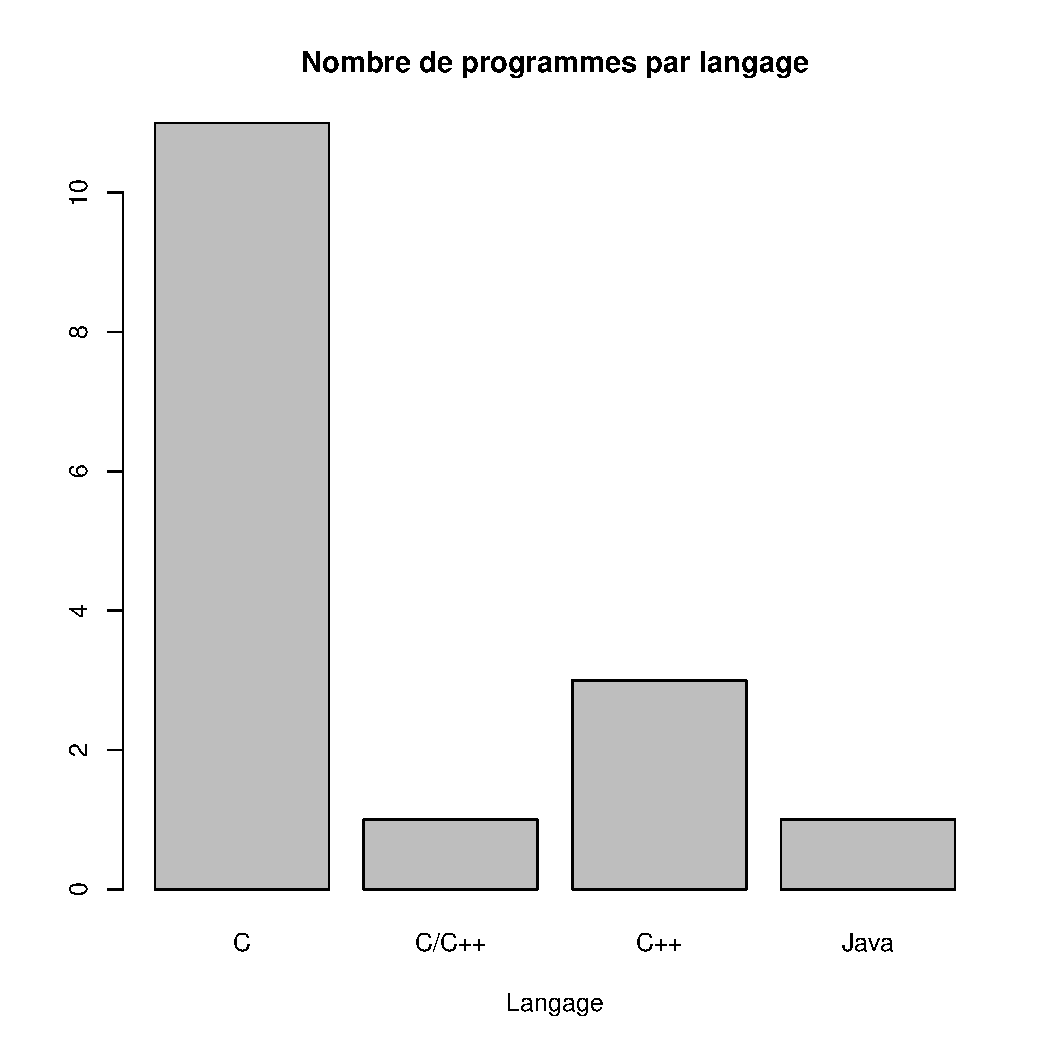
\includegraphics[width=\linewidth]{figures/prog_lang.pdf}
  \caption{}\label{fig:prog_lang}
  \endminipage\hfill
  \minipage{0.48\textwidth}
  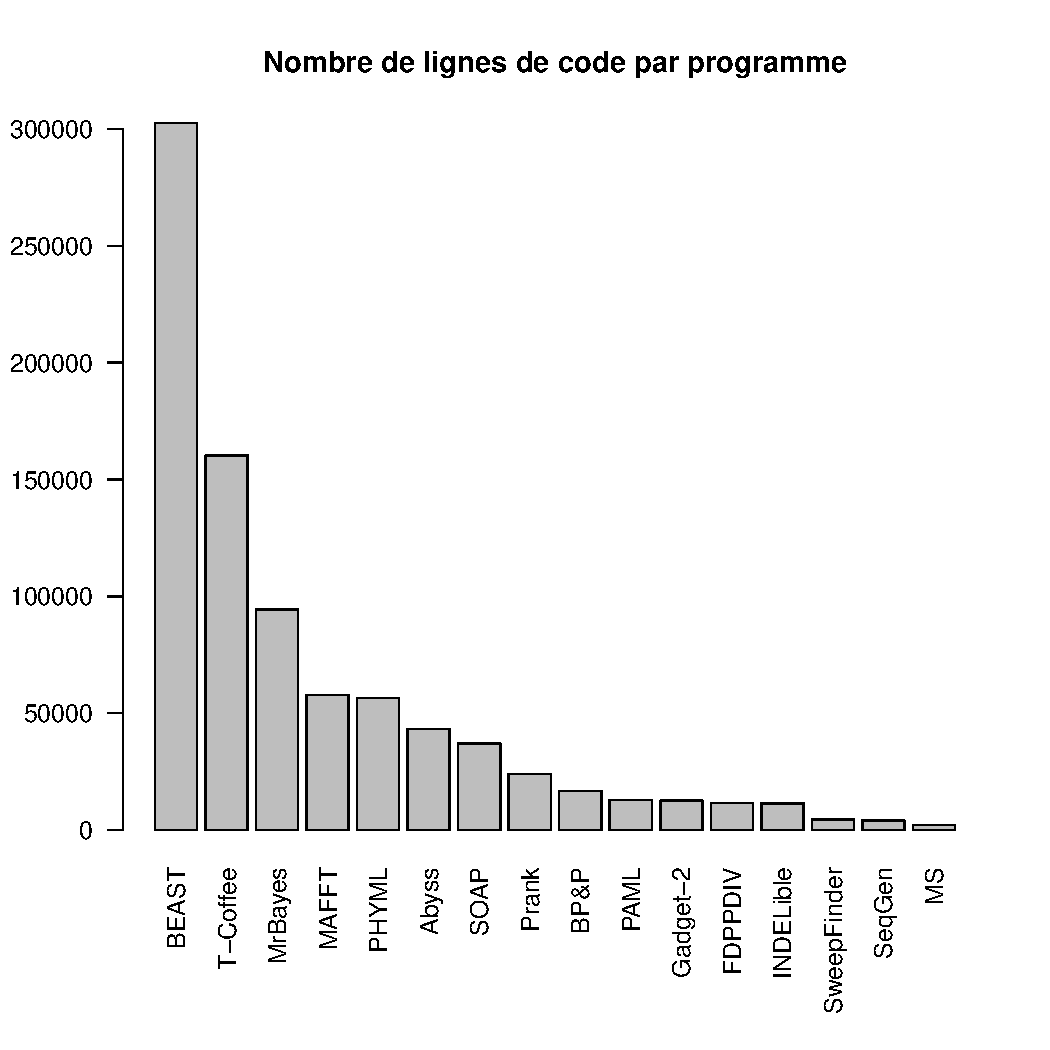
\includegraphics[width=\linewidth]{figures/lin_prog.pdf}
  \caption{}\label{fig:lin_prog}
  \endminipage\hfill
\end{figure}

\begin{figure}[!h]
  \minipage{0.48\textwidth}
  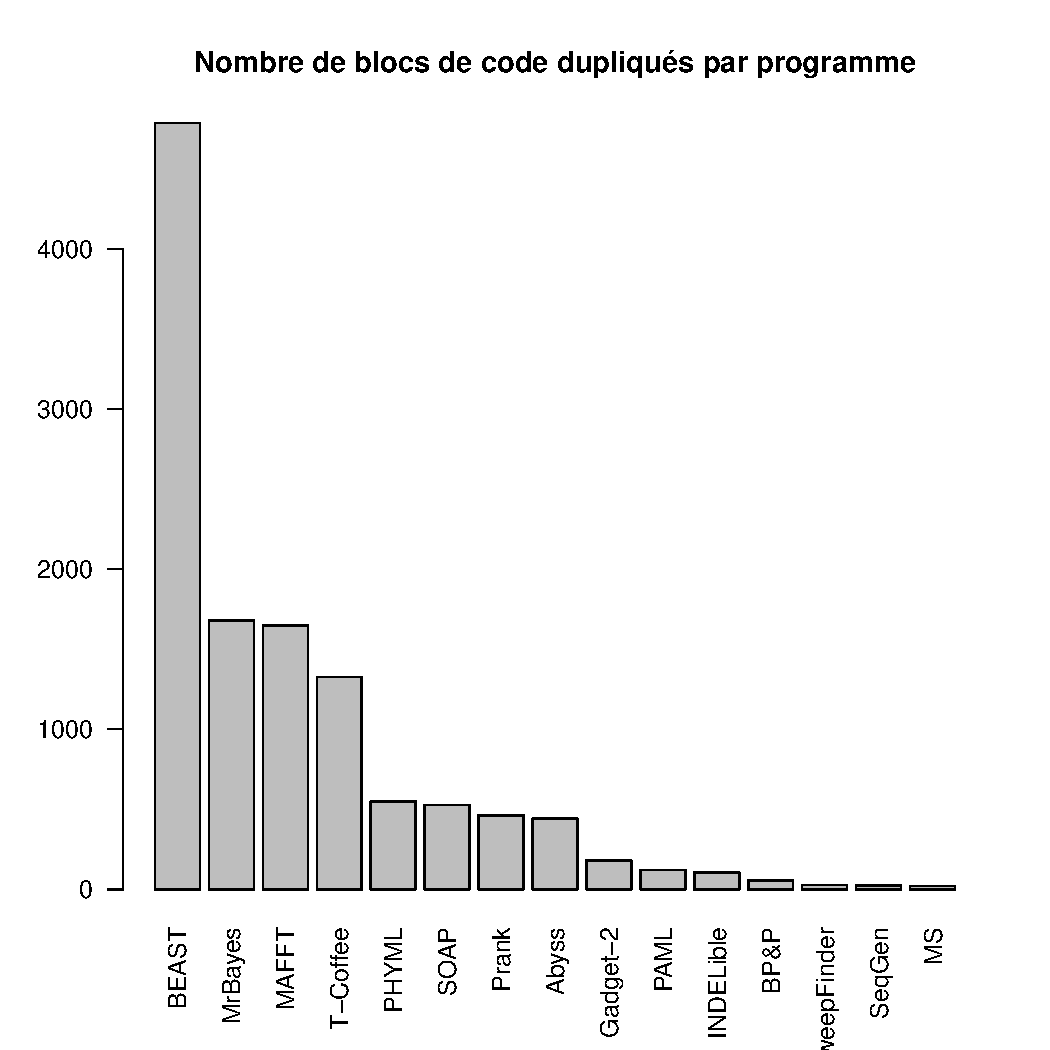
\includegraphics[width=\linewidth]{figures/dbl_prog.pdf}
  \caption{}\label{fig:dbl_prog}
  \endminipage\hfill
  \minipage{0.48\textwidth}
  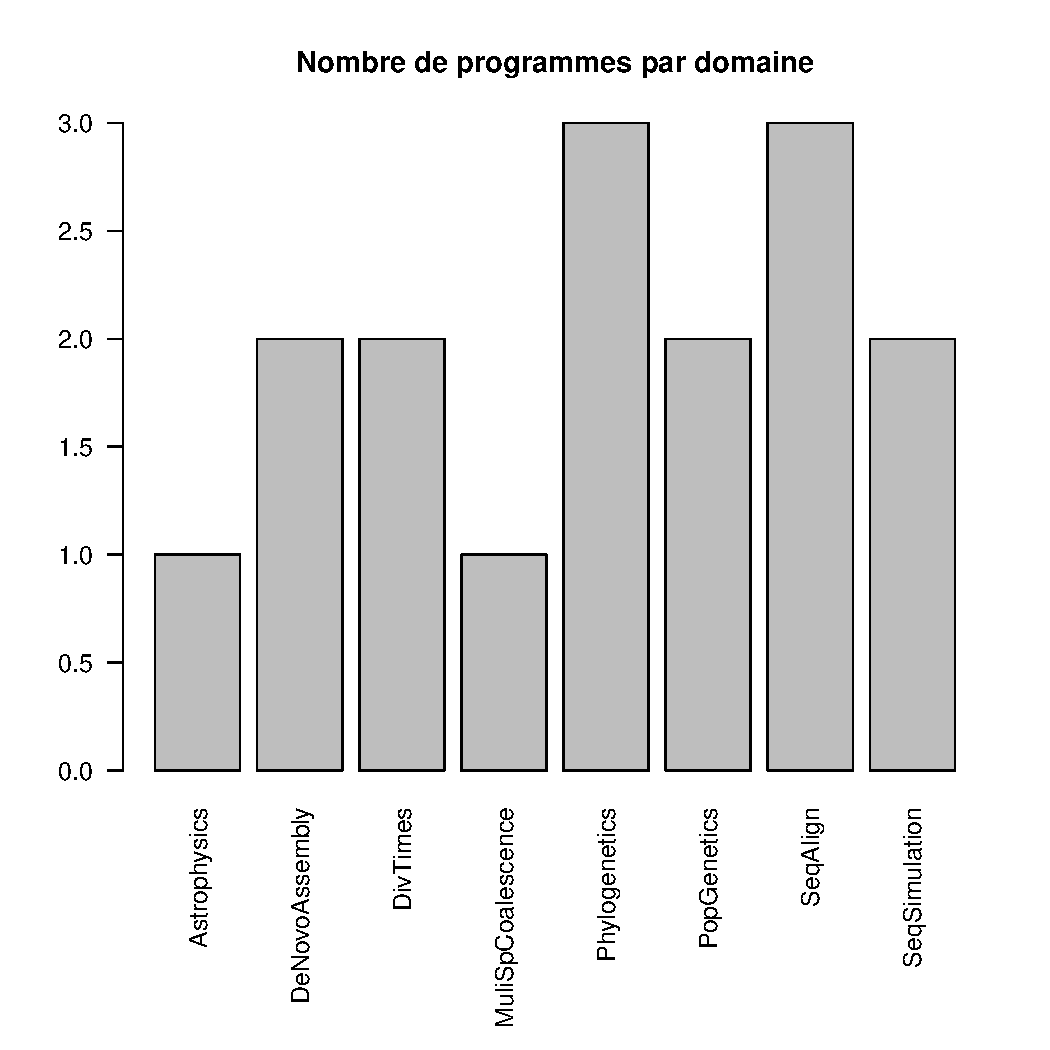
\includegraphics[width=\linewidth]{figures/prog_dom.pdf}
  \caption{}\label{fig:prog_dom}
  \endminipage\hfill
\end{figure}
